% Fuente: Industriales/Capitulos/Tema3_Calculo_Diferencial.tex
% SHA-256 original: 9940b67fcbc0878362525e23e3fdd873ead822063f8691994d6b85b559e14489
\bloque{derivadas-integrales}
\tema{calculo-diferencial}{Cálculo diferencial}
\dificultad{1}

\section{Cálculo diferencial - fragmento 1}
\textbf{Cálculo diferencial}

En el capítulo anterior estudiamos cómo describir una función y cómo analizar su comportamiento mediante límites y continuidad. El cálculo diferencial añade una pregunta esencial: \emph{¿cómo está cambiando una magnitud?} La derivada permite responderla localmente y, a partir de esa información, deducir propiedades globales de una función.

Esta idea admite varios registros que deben manejarse de forma coordinada. Analíticamente, la derivada se obtiene como un límite y se representa mediante una nueva función $f'$. Gráficamente, $f'(x)$ es la pendiente de la recta tangente a la gráfica de $f$ en el punto de abscisa $x$. Verbalmente, expresa la tasa instantánea de cambio de la magnitud representada por $f$. A lo largo del capítulo se trabajará de forma sistemática el paso entre estos tres registros. En ingeniería, esta traducción es tan importante como el propio cálculo simbólico: no basta con obtener una derivada; hay que saber qué información proporciona sobre el sistema que se está estudiando.

\textbf{Derivada y diferenciabilidad}

\textbf{Tasa de variación y pendiente de la recta tangente}

Sea $y=f(x)$ una magnitud que depende de otra magnitud $x$. Si $x$ cambia desde $x_0$ hasta $x_0+h$, el incremento de la variable independiente es
\[
\Delta x=h,
\]
y el correspondiente incremento de la función es
\[
\Delta y=f(x_0+h)-f(x_0).
\]

\begin{definition}[Tasa de variación media]
La \emph{tasa de variación media} de $f$ entre $x_0$ y $x_0+h$, con $h\neq0$, es
\[
\frac{\Delta y}{\Delta x}
=
\frac{f(x_0+h)-f(x_0)}{h}.
\]
\end{definition}


\section{Cálculo diferencial - fragmento 2}
Desde el punto de vista geométrico, este cociente es la pendiente de la recta secante que pasa por
\[
P=(x_0,f(x_0)),
\qquad
Q=(x_0+h,f(x_0+h)).
\]
Si hacemos que $Q$ se aproxime a $P$, es decir, $h\to0$, la secante tiende, cuando existe el límite correspondiente, a la recta tangente.

\begin{figure}[htbp]
\centering
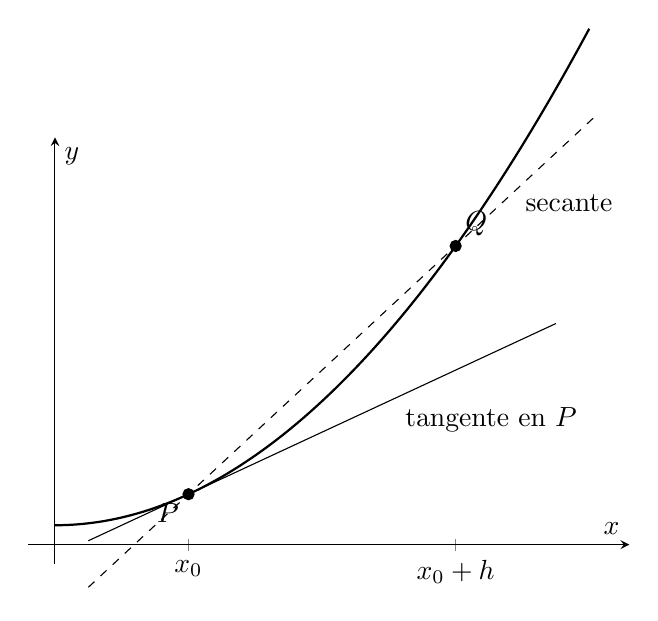
\begin{tikzpicture}
\begin{axis}[
    width=.76\textwidth,
    height=7cm,
    axis lines=middle,
    xmin=-.2,xmax=4.3,
    ymin=-.5,ymax=10.5,
    xlabel={$x$},ylabel={$y$},
    samples=150,
    xtick={1,3},
    xticklabels={$x_0$,$x_0+h$},
    ytick=\empty,
    clip=false
]
\addplot[thick,domain=0:4] {0.8*x^2+0.5};
\addplot[dashed,domain=.25:4.05] {3.2*x-1.9};
\addplot[domain=.25:3.75] {1.6*x-0.3};
\addplot[only marks,mark=*] coordinates {(1,1.3) (3,7.7)};
\node[anchor=north east] at (axis cs:1,1.3) {$P$};
\node[anchor=south west] at (axis cs:3,7.7) {$Q$};
\node[anchor=south west] at (axis cs:3.45,8.34) {secante};
\node[anchor=north west] at (axis cs:2.55,3.78) {tangente en $P$};
\end{axis}
\end{tikzpicture}
\caption{La pendiente de las secantes se aproxima a la pendiente de la tangente cuando $Q$ se acerca a $P$.}

\end{figure}

Esta misma construcción aparece al estudiar movimiento. Si $s(t)$ indica la posición de un móvil en el instante $t$, entonces
\[
\frac{s(t_0+h)-s(t_0)}{h}
\]
es la velocidad media durante el intervalo de tiempo $[t_0,t_0+h]$. Cuando el intervalo se hace arbitrariamente pequeño, obtenemos la velocidad instantánea.

\begin{definition}[Derivada en un punto]
Sea $f:D\subseteq\mathbb{R}\to\mathbb{R}$ y sea $x_0$ un punto interior de $D$. La \emph{derivada de $f$ en $x_0$} es, si existe y es finita, el límite
\[
f'(x_0)=\lim_{h\to0}\frac{f(x_0+h)-f(x_0)}{h}.
\]
Cuando este límite existe, se dice que $f$ es \emph{derivable} o \emph{diferenciable} en $x_0$.
\end{definition}

El cociente
\[
\frac{f(x_0+h)-f(x_0)}{h}
\]
se denomina \emph{cociente incremental}. La derivada es, por tanto, el límite de las tasas de variación medias cuando el incremento de la variable independiente tiende a cero.


\section{Cálculo diferencial - fragmento 3}
\begin{example}[De la velocidad media a la instantánea]
La posición de un carro móvil a lo largo de una guía viene dada por
\[
s(t)=t^2+2t\qquad (s\text{ en metros},\ t\text{ en segundos}).
\]
La velocidad media entre $t=2$ y $t=2+h$ es
\[
\frac{s(2+h)-s(2)}{h}
=
\frac{(2+h)^2+2(2+h)-8}{h}
=
6+h.
\]
Al hacer $h\to0$,
\[
v(2)=s'(2)=6\ \mathrm{m/s}.
\]
La misma cantidad tiene tres lecturas: analíticamente es $s'(2)=6$; gráficamente es la pendiente de la tangente a la gráfica posición--tiempo en $t=2$; verbalmente significa que, en ese instante, la posición aumenta aproximadamente $6$ metros por cada segundo adicional.
\end{example}

\begin{solvedexercise}
Calcular, utilizando exclusivamente la definición, la derivada de
\[
f(x)=x^2
\]
en un punto arbitrario $x_0$.

\textbf{Resolución.}\par\smallskip
Partimos del cociente incremental:
\[
\frac{f(x_0+h)-f(x_0)}{h}
=
\frac{(x_0+h)^2-x_0^2}{h}
=
\frac{2x_0h+h^2}{h}
=2x_0+h.
\]
Por tanto,
\[
f'(x_0)=\lim_{h\to0}(2x_0+h)=2x_0.
\]
Como $x_0$ es arbitrario, podemos escribir
\[
f'(x)=2x.
\]
\end{solvedexercise}

\textbf{Interpretación geométrica, física y unidades}

Si $f$ es derivable en $x_0$, la pendiente de la recta tangente a la gráfica $y=f(x)$ en el punto $(x_0,f(x_0))$ es $f'(x_0)$. Por tanto, su ecuación es
\[
y-f(x_0)=f'(x_0)(x-x_0).
\]

\begin{definition}[Recta tangente]
Si $f$ es derivable en $x_0$, la recta tangente a la gráfica de $f$ en $(x_0,f(x_0))$ es
\[
\boxed{\ y=f(x_0)+f'(x_0)(x-x_0).\ }
\]
\end{definition}

\begin{example}
Para
\[
f(x)=x^2+1,
\]
tenemos $f'(x)=2x$. En $x_0=2$,
\[
f(2)=5,
\qquad
f'(2)=4.
\]
La recta tangente es
\[
y-5=4(x-2),
\qquad\text{es decir,}\qquad
 y=4x-3.
\]
El signo positivo de la pendiente indica, además, que la función está creciendo alrededor de $x=2$.
\end{example}

La unidad de la derivada se obtiene dividiendo la unidad de la magnitud dependiente entre la unidad de la variable independiente. Esta observación es esencial para interpretar resultados en problemas aplicados.


\section{Cálculo diferencial - fragmento 4}
\begin{example}[Velocidad de calentamiento]
La temperatura de una pieza durante un proceso térmico se modela por
\[
T(t)=20+80\bigl(1-e^{-0.05t}\bigr),
\]
donde $T$ se mide en grados Celsius y $t$ en minutos. Su derivada es
\[
T'(t)=4e^{-0.05t}.
\]
Por tanto, $T'(10)$ se mide en $^{\circ}\mathrm{C}/\mathrm{min}$ y expresa la velocidad instantánea con la que cambia la temperatura a los diez minutos. Como $T'(t)>0$, la temperatura aumenta; como el valor de $T'(t)$ disminuye con el tiempo, el calentamiento se hace progresivamente más lento.
\end{example}

Cuando $f(x_0)\neq0$, también puede resultar útil comparar la tasa de cambio con el tamaño de la propia magnitud.

\begin{definition}[Tasa relativa de cambio]
La \emph{tasa relativa de cambio} de $f$ en $x_0$ es
\[
\frac{f'(x_0)}{f(x_0)}.
\]
Multiplicada por $100$, se interpreta como porcentaje instantáneo de cambio por unidad de la variable independiente.
\end{definition}

Por ejemplo, si la potencia generada por una instalación es $P(t)$, el cociente $P'(t)/P(t)$ indica la variación instantánea de la potencia en relación con el nivel de producción existente en ese instante.

\textbf{Función derivada, notación y diferenciabilidad}

Si $f$ es derivable en todos los puntos de un intervalo, podemos considerar una nueva función que a cada punto le asigna la pendiente de la tangente correspondiente.

\begin{definition}[Función derivada]
La \emph{función derivada} de $f$ es
\[
f':x\longmapsto f'(x).
\]
\end{definition}

Utilizaremos indistintamente las notaciones
\[
f'(x),
\qquad
y',
\qquad
\frac{dy}{dx},
\qquad
\frac{df}{dx}.
\]
Cuando la variable independiente es el tiempo también es habitual, especialmente en mecánica, la notación de Newton
\[
\dot y(t)=\frac{dy}{dt}.
\]

La derivabilidad es una propiedad más fuerte que la continuidad.


\section{Cálculo diferencial - fragmento 5}
\begin{theorem}[Derivabilidad implica continuidad]
Si $f$ es derivable en $x_0$, entonces $f$ es continua en $x_0$.
\end{theorem}

\begin{proof}
Para $x=x_0+h$,
\[
f(x_0+h)-f(x_0)
=
\frac{f(x_0+h)-f(x_0)}{h}\,h.
\]
Si $f$ es derivable en $x_0$, el primer factor tiende a $f'(x_0)$ y el segundo a $0$. Por tanto,
\[
\lim_{h\to0}\bigl(f(x_0+h)-f(x_0)\bigr)=0,
\]
de donde
\[
\lim_{x\to x_0}f(x)=f(x_0).
\]
\end{proof}

El recíproco es falso: una función puede ser continua y no derivable. El ejemplo más sencillo es $f(x)=|x|$ en $x=0$. Sus derivadas laterales son
\[
f'_-(0)=-1,
\qquad
f'_+(0)=1,
\]
y, al no coincidir, $f'(0)$ no existe. Gráficamente aparece un punto anguloso.

También pueden aparecer tangentes verticales. En ese caso el cociente incremental puede tender a $+\infty$ o $-\infty$, pero, con la definición anterior, no diremos que existe una derivada real finita.

\begin{solvedexercise}
Estudiar la derivabilidad de
\[
f(x)=
\begin{cases}
ax+1, & x\leq1,\\
x^2+b, & x>1,
\end{cases}
\]
y determinar $a$ y $b$ para que sea derivable en todo $\mathbb{R}$.

\textbf{Resolución.}\par\smallskip
Sólo hay que estudiar $x=1$. Para que la función sea derivable debe ser primero continua:
\[
a+1=1+b,
\]
es decir,
\[
b=a.
\]
Las derivadas laterales son
\[
f'_-(1)=a,
\qquad
f'_+(1)=2.
\]
La derivabilidad exige $a=2$, y por continuidad $b=2$. Por tanto,
\[
\boxed{a=b=2}.
\]
\end{solvedexercise}

\paragraph{Comprobación con Mathematica.}
La función \texttt{D} calcula derivadas simbólicas. Por ejemplo,
\begin{mathematicacode}
D[x^2 Exp[-x], x]
\end{mathematicacode}
Para visualizar simultáneamente una función y su recta tangente en $x=2$ puede utilizarse, una vez calculada la derivada,
\begin{mathematicacode}
f[x_] := x^2 + 1
Plot[{f[x], f[2] + f'[2] (x - 2)}, {x, -1, 4}]
\end{mathematicacode}
El gráfico sirve para comprobar la interpretación geométrica; la pendiente y la ecuación de la tangente deben haberse obtenido y justificado analíticamente.


\section{Cálculo diferencial - fragmento 6}
\textbf{Cálculo de derivadas}

La definición permite calcular cualquier derivada siempre que el límite correspondiente pueda resolverse. Sin embargo, repetir ese proceso para cada función sería poco eficiente. A partir de la definición se obtienen reglas que permiten derivar directamente la mayoría de las funciones elementales.

\textbf{Reglas básicas y derivadas elementales}

Sean $f$ y $g$ funciones derivables y $\lambda\in\mathbb{R}$. Se verifican las reglas
\[
(f\pm g)'=f'\pm g',
\]
\[
(\lambda f)'=\lambda f',
\]
\[
(fg)'=f'g+fg',
\]
y, siempre que $g(x)\neq0$,
\[
\left(\frac{f}{g}\right)'
=
\frac{f'g-fg'}{g^2}.
\]

La siguiente tabla recoge las derivadas que utilizaremos con mayor frecuencia:

\begin{center}

\begin{tabular}{@{}ll@{}}
\toprule
Función & Derivada \\
\midrule
$c$ & $0$ \\
$x^n$ & $nx^{n-1}$ \\
$e^x$ & $e^x$ \\
$a^x$ & $a^x\ln a$ \\
$\ln x$ & $1/x$ \\
$\log_a x$ & $1/(x\ln a)$ \\
$\sin x$ & $\cos x$ \\
$\cos x$ & $-\sin x$ \\
$\tan x$ & $1/\cos^2x$ \\
$\arcsin x$ & $1/\sqrt{1-x^2}$ \\
$\arccos x$ & $-1/\sqrt{1-x^2}$ \\
$\arctan x$ & $1/(1+x^2)$ \\
\bottomrule
\end{tabular}
\end{center}

Para potencias reales, la regla
\[
\frac{d}{dx}x^r=rx^{r-1}
\]
se aplica en los intervalos en los que la función y la expresión resultante estén definidas.

\begin{solvedexercise}
Derivar
\[
f(x)=\frac{x^2e^x}{1+x^2}.
\]

\textbf{Resolución.}\par\smallskip
Tomamos
\[
u(x)=x^2e^x,
\qquad
v(x)=1+x^2.
\]
Entonces
\[
u'(x)=2xe^x+x^2e^x=e^x(2x+x^2),
\qquad
v'(x)=2x.
\]
Por la regla del cociente,
\[
f'(x)=
\frac{e^x(2x+x^2)(1+x^2)-2x^3e^x}{(1+x^2)^2}.
\]
Sacando factor común $e^x$ y simplificando,
\[
\boxed{
f'(x)=\frac{e^x(x^4+x^2+2x)}{(1+x^2)^2}
}.
\]
La forma no simplificada también es correcta y, en algunos problemas, puede ser más útil para interpretar el origen de cada término.
\end{solvedexercise}


\section{Cálculo diferencial - fragmento 7}
\textbf{Funciones compuestas y regla de la cadena}

Muchas magnitudes dependen de otras a través de varias etapas. Si $u=g(x)$ e $y=f(u)$, entonces
\[
y=(f\circ g)(x)=f(g(x)).
\]

\begin{theorem}[Regla de la cadena]
Si $g$ es derivable en $x$ y $f$ es derivable en $g(x)$, entonces $f\circ g$ es derivable en $x$ y
\[
(f\circ g)'(x)=f'(g(x))g'(x).
\]
En notación de Leibniz,
\[
\frac{dy}{dx}=\frac{dy}{du}\frac{du}{dx}.
\]
\end{theorem}

La regla de la cadena expresa matemáticamente la propagación de una tasa de cambio a través de dependencias sucesivas.

\begin{example}[Variación de una resistencia con la temperatura]
Supongamos que la resistencia eléctrica de un conductor depende de la temperatura mediante
\[
R(T)=R_0\bigl(1+\alpha(T-T_0)\bigr),
\]
y que la temperatura evoluciona con el tiempo según $T=T(t)$. Entonces
\[
\frac{dR}{dt}
=
\frac{dR}{dT}\frac{dT}{dt}
=
R_0\alpha\,T'(t).
\]
La fórmula separa dos efectos: la sensibilidad de la resistencia a la temperatura y la velocidad con la que cambia la temperatura.
\end{example}

\begin{example}
Para
\[
f(x)=\sin\!\bigl((1+x^2)^3\bigr),
\]
aplicamos sucesivamente la regla de la cadena:
\[
f'(x)
=
\cos\!\bigl((1+x^2)^3\bigr)\,3(1+x^2)^2\,2x.
\]
Por tanto,
\[
\boxed{
f'(x)=6x(1+x^2)^2\cos\!\bigl((1+x^2)^3\bigr)
}.
\]
\end{example}

\textbf{Derivación implícita y logarítmica}

No siempre una relación entre variables viene dada explícitamente como $y=f(x)$. Si $x$ e $y$ están ligados por una ecuación
\[
F(x,y)=0,
\]
podemos derivar ambos miembros respecto de $x$, teniendo en cuenta que $y=y(x)$.

\begin{example}[Derivación implícita]
Sea
\[
x^2+xy+y^2=7.
\]
Derivando respecto de $x$,
\[
2x+y+xy'+2yy'=0.
\]
Agrupando los términos que contienen $y'$,
\[
(x+2y)y'=-(2x+y),
\]
y, siempre que $x+2y\neq0$,
\[
\boxed{
y'=-\frac{2x+y}{x+2y}
}.
\]
No ha sido necesario despejar previamente $y$.
\end{example}


\section{Cálculo diferencial - fragmento 8}
\begin{solvedexercise}
Mostrar que las tangentes en el origen a las curvas
\[
5y-2x+y^3-x^2y=0
\]
y
\[
2y+5x+x^4-x^3y^2=0
\]
son perpendiculares.

\textbf{Resolución.}\par\smallskip
Para la primera curva, derivando implícitamente,
\[
5y'-2+3y^2y'-2xy-x^2y'=0.
\]
En $(0,0)$,
\[
5y'(0)-2=0,
\qquad
y'(0)=\frac25.
\]
Para la segunda,
\[
2y'+5+4x^3-3x^2y^2-2x^3yy'=0.
\]
En el origen,
\[
2y'(0)+5=0,
\qquad
y'(0)=-\frac52.
\]
El producto de las pendientes es
\[
\frac25\left(-\frac52\right)=-1,
\]
por lo que las tangentes son perpendiculares.
\end{solvedexercise}

La derivación logarítmica resulta especialmente útil cuando la variable aparece simultáneamente en una base y en un exponente, o cuando una expresión está formada por productos y cocientes de muchas potencias.

Si $y=f(x)>0$, tomamos logaritmos:
\[
\ln y=\ln f(x),
\]
derivamos implícitamente y despejamos $y'$.

\begin{example}[Derivación logarítmica]
Sea
\[
y=x^{\sin x},
\qquad x>0.
\]
Tomando logaritmos,
\[
\ln y=\sin x\,\ln x.
\]
Derivando,
\[
\frac{y'}{y}
=
\cos x\,\ln x+\frac{\sin x}{x}.
\]
Por tanto,
\[
\boxed{
y'=x^{\sin x}\left(\cos x\,\ln x+\frac{\sin x}{x}\right)
}.
\]
\end{example}

\textbf{Derivadas sucesivas}

Si $f'$ es derivable, su derivada se denomina \emph{segunda derivada} de $f$ y se denota
\[
f''(x)=\frac{d^2f}{dx^2}.
\]
De forma sucesiva se definen
\[
f'''(x),
\qquad
f^{(4)}(x),
\qquad
\ldots,
\qquad
f^{(n)}(x)=\frac{d^nf}{dx^n}.
\]

Las derivadas de orden superior describen cambios de las propias tasas de cambio. Si $s(t)$ es la posición de un móvil,
\[
v(t)=s'(t)
\]
es su velocidad y
\[
a(t)=s''(t)
\]
es su aceleración. Por tanto, $s$, $s'$ y $s''$ no son tres objetos aislados: representan distintos niveles de variación de un mismo fenómeno.


\section{Cálculo diferencial - fragmento 9}
\begin{solvedexercise}
La posición de un mecanismo viene dada por
\[
s(t)=2\sin(3t),
\]
con $s$ en centímetros y $t$ en segundos. Calcular velocidad y aceleración, y relacionar sus signos con el movimiento cuando $t=\pi/18$.

\textbf{Resolución.}\par\smallskip
Tenemos
\[
v(t)=s'(t)=6\cos(3t),
\qquad
a(t)=s''(t)=-18\sin(3t).
\]
Para $t=\pi/18$ se tiene $3t=\pi/6$, y por tanto
\[
v\!\left(\frac{\pi}{18}\right)=3\sqrt3>0,
\]
\[
a\!\left(\frac{\pi}{18}\right)=-9<0.
\]
La posición está aumentando en ese instante, pero la velocidad está disminuyendo. El sistema se mueve en el sentido positivo mientras experimenta una aceleración en sentido contrario al movimiento.
\end{solvedexercise}

\textbf{Teoremas fundamentales y aproximación}

Las reglas anteriores permiten calcular derivadas. Los resultados de esta sección explican qué consecuencias tienen esas derivadas sobre el comportamiento de una función y permiten utilizar información local para obtener conclusiones globales.

\textbf{Teoremas de Rolle y del valor medio}

Comenzamos con una condición necesaria para que una función derivable tenga un extremo interior.

\begin{theorem}[Teorema de Fermat]
Sea $f$ derivable en un punto interior $x_0$ de su dominio. Si $f$ tiene en $x_0$ un máximo o un mínimo relativo, entonces
\[
f'(x_0)=0.
\]
\end{theorem}

El recíproco no es cierto: $f'(x_0)=0$ no garantiza que exista un extremo. Por ejemplo, $f(x)=x^3$ satisface $f'(0)=0$ y, sin embargo, es estrictamente creciente alrededor de $0$.

\begin{theorem}[Teorema de Rolle]
Sea $f:[a,b]\to\mathbb{R}$ continua en $[a,b]$ y derivable en $]a,b[$. Si
\[
f(a)=f(b),
\]
entonces existe al menos un punto $c\in]a,b[$ tal que
\[
f'(c)=0.
\]
\end{theorem}

Geométricamente, si una curva derivable parte y termina a la misma altura, debe tener al menos una tangente horizontal entre ambos extremos.

\begin{theorem}[Teorema del valor medio]
Sea $f:[a,b]\to\mathbb{R}$ continua en $[a,b]$ y derivable en $]a,b[$. Entonces existe al menos un punto $c\in]a,b[$ tal que
\[
f'(c)=\frac{f(b)-f(a)}{b-a}.
\]
\end{theorem}


\section{Cálculo diferencial - fragmento 10}
El teorema afirma que, bajo las hipótesis indicadas, alguna tasa instantánea de cambio coincide con la tasa media de cambio en todo el intervalo.

\begin{example}[Interpretación cinemática]
Un vehículo recorre $180$ km en dos horas y su posición es una función continua del tiempo y derivable durante el trayecto. Su velocidad media es
\[
\frac{180}{2}=90\ \mathrm{km/h}.
\]
El Teorema del Valor Medio garantiza que existe al menos un instante del recorrido en el que la velocidad instantánea es exactamente $90\ \mathrm{km/h}$.
\end{example}

\begin{solvedexercise}
Comprobar que la función
\[
f(x)=x^2-4x+3
\]
satisface las hipótesis del Teorema de Rolle en $[1,3]$ y hallar todos los puntos cuya existencia garantiza el teorema.

\textbf{Resolución.}\par\smallskip
La función es polinómica, luego es continua en $[1,3]$ y derivable en $]1,3[$. Además,
\[
f(1)=0=f(3).
\]
Por Rolle existe al menos $c\in]1,3[$ con $f'(c)=0$. Como
\[
f'(x)=2x-4,
\]
se obtiene
\[
2c-4=0,
\qquad
\boxed{c=2}.
\]
\end{solvedexercise}

\textbf{Regla de L'Hôpital}

La Regla de L'Hôpital permite resolver determinadas indeterminaciones de tipo $0/0$ o $\infty/\infty$ utilizando derivadas.

\begin{theorem}[Regla de L'Hôpital]
Sean $f$ y $g$ derivables en un entorno perforado de $a$, con $g'(x)\neq0$ en dicho entorno. Supongamos que
\[
\lim_{x\to a}f(x)=\lim_{x\to a}g(x)=0
\]
o que $|f(x)|$ y $|g(x)|$ tienden a infinito. Si existe
\[
\lim_{x\to a}\frac{f'(x)}{g'(x)}=L,
\]
con $L\in\mathbb{R}\cup\{\pm\infty\}$, entonces, bajo estas hipótesis,
\[
\lim_{x\to a}\frac{f(x)}{g(x)}=L.
\]
El resultado también se aplica a límites laterales y a límites cuando $x\to\pm\infty$.
\end{theorem}

La regla sólo debe utilizarse después de comprobar que se está ante una de las indeterminaciones permitidas. No es una regla general para derivar numerador y denominador en cualquier cociente.


\section{Cálculo diferencial - fragmento 11}
\begin{example}
Calcular
\[
\lim_{x\to0}\frac{e^{2x}-1}{x}.
\]
La sustitución directa produce $0/0$. Aplicando L'Hôpital,
\[
\lim_{x\to0}\frac{e^{2x}-1}{x}
=
\lim_{x\to0}\frac{2e^{2x}}{1}
=2.
\]
\end{example}

Las indeterminaciones $0\cdot\infty$, $\infty-\infty$ y las indeterminaciones exponenciales deben transformarse previamente en un cociente de tipo $0/0$ o $\infty/\infty$, o bien tratarse tomando logaritmos cuando corresponda.

\begin{solvedexercise}
Calcular
\[
\lim_{x\to0^+}x\ln x.
\]

\textbf{Resolución.}\par\smallskip
La expresión es de tipo $0\cdot(-\infty)$. La escribimos como
\[
x\ln x=\frac{\ln x}{1/x}.
\]
Ahora tenemos una indeterminación $(-\infty)/(+\infty)$. Aplicando L'Hôpital,
\[
\lim_{x\to0^+}\frac{1/x}{-1/x^2}
=
\lim_{x\to0^+}(-x)=0.
\]
Por tanto,
\[
\boxed{\lim_{x\to0^+}x\ln x=0}.
\]
\end{solvedexercise}

\textbf{Aproximación lineal y polinomio de Taylor}

La derivabilidad implica que, a escala suficientemente pequeña, una función se comporta aproximadamente como una función lineal. Si $f$ es derivable en $x_0$, entonces
\[
f(x_0+h)=f(x_0)+f'(x_0)h+o(h),
\qquad h\to0.
\]
Por ello, para $x$ próximo a $x_0$,
\[
\boxed{
f(x)\approx f(x_0)+f'(x_0)(x-x_0)
}.
\]
El miembro derecho es precisamente la ordenada de la recta tangente.

\begin{example}[Estimación de una variación]
El radio de una pieza circular pasa de $10$ cm a $10.1$ cm. Para
\[
A(r)=\pi r^2,
\]
la variación exacta es
\[
\Delta A=A(10.1)-A(10)=2.01\pi\ \mathrm{cm}^2.
\]
La aproximación lineal proporciona
\[
\Delta A\approx A'(10)\,\Delta r
=20\pi\cdot0.1
=2\pi\ \mathrm{cm}^2.
\]
La diferencia es pequeña porque el incremento del radio es pequeño respecto de su valor inicial.
\end{example}

La aproximación puede mejorarse incorporando derivadas de orden superior.

\begin{definition}[Polinomio de Taylor]
Supongamos que $f$ tiene derivadas hasta orden $n$ en un entorno de $x_0$. El \emph{polinomio de Taylor de orden $n$ de $f$ centrado en $x_0$} es
\[
P_n(x)
=
\sum_{k=0}^n\frac{f^{(k)}(x_0)}{k!}(x-x_0)^k.
\]
Es decir,
\begin{align*}
P_n(x)={}&f(x_0)+f'(x_0)(x-x_0)
+\frac{f''(x_0)}{2!}(x-x_0)^2\\
&+\cdots
+\frac{f^{(n)}(x_0)}{n!}(x-x_0)^n.
\end{align*}
\end{definition}


\section{Cálculo diferencial - fragmento 12}
Cuando $x_0=0$ se habla también de \emph{polinomio de Maclaurin}.

\begin{theorem}[Taylor con resto de Lagrange]
Si $f$ tiene $n+1$ derivadas continuas en un intervalo que contiene a $x_0$ y a $x$, existe un punto $\xi$ entre $x_0$ y $x$ tal que
\[
f(x)=P_n(x)+R_n(x),
\]
donde
\[
R_n(x)=\frac{f^{(n+1)}(\xi)}{(n+1)!}(x-x_0)^{n+1}.
\]
\end{theorem}

Este resto permite estimar el error cometido al sustituir una función por su polinomio de Taylor.

\begin{example}
Obtener el polinomio de Maclaurin de orden $3$ de $e^x$. Como todas las derivadas de $e^x$ coinciden con $e^x$,
\[
f^{(k)}(0)=1
\]
para todo $k$. Por tanto,
\[
\boxed{
P_3(x)=1+x+\frac{x^2}{2}+\frac{x^3}{6}
}.
\]
Cerca de $x=0$, este polinomio reproduce no sólo el valor y la pendiente de $e^x$, sino también sus dos siguientes niveles de variación.
\end{example}

\begin{solvedexercise}
Obtener el polinomio de Maclaurin de orden $5$ de $\sin x$ y utilizarlo para aproximar $\sin(0.2)$.

\textbf{Resolución.}\par\smallskip
Las derivadas de $\sin x$ se repiten cíclicamente. En $x=0$,
\begin{align*}
f(0)&=0, & f'(0)&=1, & f''(0)&=0,\\
f'''(0)&=-1, & f^{(4)}(0)&=0, & f^{(5)}(0)&=1.
\end{align*}
Por tanto,
\[
P_5(x)=x-\frac{x^3}{3!}+\frac{x^5}{5!}.
\]
Así,
\[
\sin(0.2)
\approx
0.2-\frac{0.2^3}{6}+\frac{0.2^5}{120}
\approx0.1986693.
\]
\end{solvedexercise}

\paragraph{Comprobación con Mathematica.}
El comando mínimo para obtener desarrollos de Taylor será \texttt{Series}. Por ejemplo,
\begin{mathematicacode}
Series[Sin[x], {x, 0, 5}]
\end{mathematicacode}
La salida incluye un término de orden que indica el resto. El objetivo de la práctica no es sustituir el cálculo de las derivadas, sino comprobar el polinomio obtenido y comparar gráficamente la función con su aproximación en distintos intervalos.

\textbf{La derivada y la forma de una función}


\section{Cálculo diferencial - fragmento 13}
La derivada no debe entenderse únicamente como una expresión que se calcula. Su utilidad principal consiste en traducir información entre distintas representaciones de una función. En esta sección estudiaremos de forma explícita las relaciones
\[
f\quad\longleftrightarrow\quad f'\quad\longleftrightarrow\quad f'',
\]
y aprenderemos a pasar del registro analítico al gráfico y al verbal, y viceversa.

\textbf{Monotonía y signo de la primera derivada}

Recordemos que una función es creciente en un intervalo si valores mayores de $x$ producen valores mayores o iguales de $f(x)$, y decreciente si ocurre lo contrario.

\begin{theorem}[Criterio de monotonía]
Sea $f$ continua en un intervalo $I$ y derivable en su interior.
\begin{itemize}
\item Si $f'(x)>0$ para todo $x$ interior a $I$, entonces $f$ es estrictamente creciente en $I$.
\item Si $f'(x)<0$ para todo $x$ interior a $I$, entonces $f$ es estrictamente decreciente en $I$.
\item Si $f'(x)=0$ para todo $x$ interior a $I$, entonces $f$ es constante en $I$.
\end{itemize}
Además, si $f$ es creciente y derivable en un punto interior $x$, entonces $f'(x)\geq0$; si es decreciente, $f'(x)\leq0$.
\end{theorem}

La información puede leerse en tres registros:

\begin{center}

\begin{tabularx}{\textwidth}{@{}>{\bfseries}lXXX@{}}
\toprule
 & Registro analítico & Registro gráfico & Registro verbal \\
\midrule
$f'(x)>0$ & La derivada es positiva & La tangente tiene pendiente positiva & $f$ aumenta al aumentar $x$ \\
$f'(x)<0$ & La derivada es negativa & La tangente tiene pendiente negativa & $f$ disminuye al aumentar $x$ \\
$f'(x)=0$ & Punto estacionario & Tangente horizontal & La variación instantánea es nula \\
$|f'(x)|$ grande & Gran valor absoluto de la derivada & Gráfica localmente muy inclinada & La magnitud cambia rápidamente \\
$|f'(x)|$ pequeño & Derivada próxima a cero & Gráfica localmente poco inclinada & La magnitud cambia lentamente \\
\bottomrule
\end{tabularx}
\end{center}


\section{Cálculo diferencial - fragmento 14}
La fila $f'(x)=0$ requiere atención: una tangente horizontal no implica necesariamente un máximo o un mínimo. Puede tratarse, por ejemplo, de un punto de inflexión horizontal.

\begin{example}[Del registro analítico al gráfico]
Sea
\[
f(x)=x^3-3x.
\]
Entonces
\[
f'(x)=3x^2-3=3(x-1)(x+1).
\]
El signo de $f'$ es
\[
\begin{array}{c|ccccc}
x & ]-\infty,-1[ & -1 & ]-1,1[ & 1 & ]1,+\infty[\\
\hline
f'(x) & + & 0 & - & 0 & +
\end{array}
\]
Por tanto, $f$ crece en $]-\infty,-1[$, decrece en $]-1,1[$ y vuelve a crecer en $]1,+\infty[$. Sin representar todavía la función, sabemos que la gráfica debe subir, alcanzar una tangente horizontal en $x=-1$, bajar hasta otra tangente horizontal en $x=1$ y volver a subir.
\end{example}

\begin{figure}[htbp]
\centering
\begin{minipage}{.48\textwidth}
\centering
\begin{tikzpicture}
\begin{axis}[
 width=\linewidth,height=6.2cm,
 axis lines=middle,xmin=-2.3,xmax=2.3,ymin=-4,ymax=4,
 xlabel={$x$},ylabel={$f(x)$},samples=150,
 xtick={-1,1},ytick=\empty
]
\addplot[thick,domain=-2.05:2.05] {x^3-3*x};
\addplot[only marks,mark=*] coordinates {(-1,2) (1,-2)};
\end{axis}
\end{tikzpicture}
\end{minipage}\hfill
\begin{minipage}{.48\textwidth}
\centering
\begin{tikzpicture}
\begin{axis}[
 width=\linewidth,height=6.2cm,
 axis lines=middle,xmin=-2.3,xmax=2.3,ymin=-4,ymax=9,
 xlabel={$x$},ylabel={$f'(x)$},samples=150,
 xtick={-1,1},ytick={0}
]
\addplot[thick,domain=-2.05:2.05] {3*x^2-3};
\end{axis}
\end{tikzpicture}
\end{minipage}
\caption{Una misma información en dos registros: la gráfica de $f$ crece exactamente donde la gráfica de $f'$ está por encima del eje horizontal.}

\end{figure}

La Figura~\ref{fig:f-y-derivada} debe leerse en ambos sentidos. Si conocemos $f$, la inclinación de su gráfica permite anticipar el signo y el tamaño de $f'$. Si conocemos $f'$, su posición respecto del eje horizontal permite reconstruir los intervalos de crecimiento y decrecimiento de $f$.


\section{Cálculo diferencial - fragmento 15}
\begin{solvedexercise}[De la derivada a la función]
Sea $f$ una función derivable cuya derivada es
\[
f'(x)=6x(x+1)(x-2).
\]
Sin calcular una expresión para $f$, estudiar los intervalos de crecimiento y decrecimiento y clasificar sus extremos relativos.

\textbf{Resolución.}\par\smallskip
Los puntos donde $f'$ se anula son
\[
x=-1,\qquad x=0,\qquad x=2.
\]
Estudiamos el signo del producto:
\[
\begin{array}{c|ccccccc}
x & ]-\infty,-1[ & -1 & ]-1,0[ & 0 & ]0,2[ & 2 & ]2,+\infty[\\
\hline
f'(x) & - & 0 & + & 0 & - & 0 & +
\end{array}
\]
Por tanto,
\begin{itemize}
\item $f$ decrece en $]-\infty,-1[$;
\item $f$ crece en $]-1,0[$;
\item $f$ decrece en $]0,2[$;
\item $f$ crece en $]2,+\infty[$.
\end{itemize}
El cambio de signo $-\to+$ en $x=-1$ indica un mínimo relativo; el cambio $+\to-$ en $x=0$ indica un máximo relativo; y el cambio $-\to+$ en $x=2$ indica otro mínimo relativo. Todo se ha deducido a partir de $f'$ sin necesidad de conocer $f$.
\end{solvedexercise}

\textbf{Extremos relativos y absolutos}

\begin{definition}[Extremos relativos]
Sea $x_0$ un punto del dominio de $f$.
\begin{itemize}
\item $f$ tiene un \emph{máximo relativo} en $x_0$ si existe un entorno de $x_0$ en el que $f(x)\leq f(x_0)$.
\item $f$ tiene un \emph{mínimo relativo} en $x_0$ si existe un entorno de $x_0$ en el que $f(x)\geq f(x_0)$.
\end{itemize}
\end{definition}

\begin{definition}[Punto crítico]
Un punto $x_0$ interior al dominio de $f$ es \emph{crítico} si
\[
f'(x_0)=0
\]
o si $f'(x_0)$ no existe.
\end{definition}

Los extremos relativos pueden aparecer en puntos donde la derivada no existe. Por ejemplo, $f(x)=|x|$ tiene un mínimo relativo y absoluto en $x=0$, aunque no es derivable en ese punto. Por ello, al buscar extremos no basta con resolver $f'(x)=0$; hay que tener en cuenta también los puntos no derivables del dominio.


\section{Cálculo diferencial - fragmento 16}
\begin{theorem}[Criterio de la primera derivada]
Sea $x_0$ un punto crítico de una función continua.
\begin{itemize}
\item Si $f'$ cambia de signo de positivo a negativo al atravesar $x_0$, entonces $f$ tiene un máximo relativo en $x_0$.
\item Si $f'$ cambia de signo de negativo a positivo al atravesar $x_0$, entonces $f$ tiene un mínimo relativo en $x_0$.
\item Si $f'$ no cambia de signo, el punto crítico no es un extremo relativo.
\end{itemize}
\end{theorem}

\begin{definition}[Extremos absolutos]
La función $f$ alcanza un \emph{máximo absoluto} en $x_M$ si
\[
f(x)\leq f(x_M)
\]
para todo $x$ de su dominio. Análogamente, alcanza un \emph{mínimo absoluto} en $x_m$ si
\[
f(x)\geq f(x_m)
\]
para todo $x$ de su dominio.
\end{definition}

\begin{theorem}[Teorema de Weierstrass]
Si $f$ es continua en un intervalo cerrado y acotado $[a,b]$, entonces alcanza en dicho intervalo un máximo absoluto y un mínimo absoluto.
\end{theorem}

Para encontrar los extremos absolutos de una función continua en $[a,b]$ se evalúa la función en los puntos críticos interiores y en los extremos $a$ y $b$, y se comparan los valores obtenidos.

\begin{solvedexercise}
Estudiar los extremos absolutos de
\[
f(x)=\frac{x+1}{x^2+1}
\]
en el intervalo $[-1,1/2]$.

\textbf{Resolución.}\par\smallskip
La función es continua en todo $\mathbb{R}$, luego alcanza máximo y mínimo absolutos en el intervalo. Su derivada es
\[
f'(x)=\frac{x^2+1-2x(x+1)}{(x^2+1)^2}
=
\frac{1-2x-x^2}{(x^2+1)^2}.
\]
Los puntos críticos satisfacen
\[
1-2x-x^2=0,
\]
es decir,
\[
x=-1\pm\sqrt2.
\]
Sólo $-1+\sqrt2$ pertenece a $[-1,1/2]$. Evaluamos
\[
f(-1)=0,
\]
\[
f\left(\frac12\right)=\frac{6}{5},
\]
y
\[
f(-1+\sqrt2)=\frac{1+\sqrt2}{2}.
\]
Como
\[
\frac{1+\sqrt2}{2}>\frac65>0,
\]
el mínimo absoluto es $0$, alcanzado en $x=-1$, y el máximo absoluto es $(1+\sqrt2)/2$, alcanzado en $x=-1+\sqrt2$.
\end{solvedexercise}


\section{Cálculo diferencial - fragmento 17}
\textbf{Segunda derivada, convexidad y puntos de inflexión}

La primera derivada informa sobre si $f$ crece o decrece. La segunda derivada informa sobre cómo cambia la pendiente de $f$.

\begin{definition}[Convexidad y concavidad]
Sea $f$ dos veces derivable en un intervalo $I$.
\begin{itemize}
\item Si $f''(x)\geq0$ en $I$, diremos que $f$ es \emph{convexa} en $I$.
\item Si $f''(x)\leq0$ en $I$, diremos que $f$ es \emph{cóncava} en $I$.
\end{itemize}
\end{definition}

En términos de $f'$, si $f''>0$, las pendientes de las tangentes aumentan; si $f''<0$, disminuyen. Esta relación permite leer la convexidad de $f$ directamente en la gráfica de $f'$.

\begin{center}

\begin{tabularx}{\textwidth}{@{}>{\bfseries}lXXX@{}}
\toprule
 & Registro analítico & Registro gráfico & Registro verbal \\
\midrule
$f''(x)>0$ & $f'$ aumenta & Las pendientes se hacen mayores & La tasa de cambio de $f$ aumenta \\
$f''(x)<0$ & $f'$ disminuye & Las pendientes se hacen menores & La tasa de cambio de $f$ disminuye \\
$f''(x)=0$ & Candidato a cambio de convexidad & Posible cambio de curvatura & La variación de la tasa puede cambiar de signo \\
\bottomrule
\end{tabularx}
\end{center}

\begin{definition}[Punto de inflexión]
Un punto $x_0$ es un \emph{punto de inflexión} de $f$ si la función cambia de convexidad al atravesarlo.
\end{definition}

Si $f''$ es continua y $x_0$ es un punto de inflexión, entonces necesariamente $f''(x_0)=0$. Sin embargo, $f''(x_0)=0$ por sí solo no garantiza un punto de inflexión. Por ejemplo, para $f(x)=x^4$ se tiene $f''(0)=0$, pero $f$ es convexa a ambos lados de $0$.


\section{Cálculo diferencial - fragmento 18}
\begin{theorem}[Criterio de la segunda derivada para extremos]
Sea $f$ dos veces derivable y supongamos que $f'(x_0)=0$.
\begin{itemize}
\item Si $f''(x_0)>0$, entonces $f$ tiene un mínimo relativo estricto en $x_0$.
\item Si $f''(x_0)<0$, entonces $f$ tiene un máximo relativo estricto en $x_0$.
\item Si $f''(x_0)=0$, el criterio no decide.
\end{itemize}
\end{theorem}

\begin{example}[Lectura verbal de la segunda derivada]
Supongamos que la temperatura de un horno aumenta durante todo un proceso, pero los operarios observan que \emph{cada minuto aumenta menos que el anterior}. Si $T(t)$ representa la temperatura, la frase se traduce en
\[
T'(t)>0
\]
porque la temperatura aumenta, y
\[
T''(t)<0
\]
porque la tasa de aumento disminuye. Gráficamente, $T$ debe ser creciente y cóncava. A su vez, la gráfica de $T'$ debe estar por encima del eje horizontal y ser decreciente.

Este ejemplo muestra que una descripción verbal suficientemente precisa permite anticipar simultáneamente la forma de $T$ y la de $T'$ sin disponer todavía de una fórmula explícita.
\end{example}

\textbf{Lectura coordinada de $f$, $f'$ y $f''$}

Para analizar correctamente una función conviene evitar una confusión frecuente: el signo de $f'$ y el crecimiento de $f'$ son informaciones distintas. El primero describe la monotonía de $f$; el segundo describe su convexidad.

Por ejemplo:
\begin{itemize}
\item si $f'>0$ y $f''>0$, la función crece y lo hace cada vez más deprisa;
\item si $f'>0$ y $f''<0$, la función crece, pero cada vez más despacio;
\item si $f'<0$ y $f''>0$, la función decrece, pero su pendiente se hace menos negativa;
\item si $f'<0$ y $f''<0$, la función decrece y su pendiente se hace cada vez más negativa.
\end{itemize}


\section{Cálculo diferencial - fragmento 19}
\begin{solvedexercise}[De un registro gráfico a uno analítico y verbal]
La siguiente gráfica representa la derivada $f'$ de una función $f$.

\begin{center}
\begin{tikzpicture}
\begin{axis}[
 width=.72\textwidth,height=6.5cm,
 axis lines=middle,
 xmin=-3.3,xmax=3.3,ymin=-4.5,ymax=5,
 xlabel={$x$},ylabel={$f'(x)$},
 xtick={-2,1},ytick={0},samples=150
]
\addplot[thick,domain=-3:3] {(x+2)*(x-1)};
\addplot[only marks,mark=*] coordinates {(-2,0) (1,0)};
\end{axis}
\end{tikzpicture}
\end{center}

Determinar, sin conocer una expresión de $f$:
\begin{enumerate}[label=\alph*)]
\item los intervalos de crecimiento y decrecimiento de $f$;
\item la naturaleza de los puntos críticos visibles;
\item los intervalos de convexidad y concavidad de $f$;
\item una descripción verbal coherente del comportamiento de $f$ cuando $x$ recorre el gráfico de izquierda a derecha.
\end{enumerate}

\textbf{Resolución.}\par\smallskip
La gráfica de $f'$ corta al eje en $x=-2$ y $x=1$.

Para $x<-2$, $f'(x)>0$, de modo que $f$ crece. Entre $-2$ y $1$, $f'(x)<0$, luego $f$ decrece. Para $x>1$, $f'(x)>0$, y $f$ vuelve a crecer. Por tanto, $x=-2$ es un máximo relativo y $x=1$ un mínimo relativo.

La gráfica de $f'$ es una parábola con vértice en
\[
x=-\frac12.
\]
Como $f'$ decrece para $x<-1/2$, se tiene $f''<0$ y $f$ es cóncava. Como $f'$ crece para $x>-1/2$, se tiene $f''>0$ y $f$ es convexa. Así, $x=-1/2$ es un punto de inflexión de $f$.

Verbalmente: la función empieza aumentando, pero su pendiente va disminuyendo; en $x=-2$ deja de aumentar y comienza a disminuir. Continúa perdiendo pendiente hasta $x=-1/2$. A partir de ahí la pendiente empieza a recuperarse, aunque todavía es negativa hasta $x=1$. En $x=1$ la función alcanza un mínimo relativo y después vuelve a crecer cada vez con mayor pendiente.
\end{solvedexercise}

Este tipo de razonamiento será especialmente importante en los ejercicios en los que se proporciona la gráfica de $f$ o de $f'$ sin una fórmula explícita.


\section{Cálculo diferencial - fragmento 20}
\textbf{Estudio de la gráfica de una función}

Para realizar un estudio cualitativo completo de una función no existe una única receta rígida, pero suele ser útil considerar, en este orden, los siguientes elementos:
\begin{enumerate}
\item dominio, cortes con los ejes, simetrías y periodicidad;
\item límites en los extremos del dominio y asíntotas;
\item continuidad y puntos no derivables;
\item signo de $f'$: monotonía y extremos;
\item signo de $f''$: convexidad, concavidad y puntos de inflexión;
\item información adicional relevante del modelo.
\end{enumerate}

La representación final debe ser coherente con \emph{toda} la información obtenida. El objetivo no es dibujar una curva aproximada al azar, sino sintetizar en un único registro gráfico las conclusiones analíticas anteriores.

\begin{solvedexercise}
Realizar un estudio de forma y esbozar la gráfica de
\[
f(x)=\frac{2(x^2-9)}{x^2-4}.
\]

\textbf{Resolución.}\par\smallskip
El dominio es
\[
\mathbb{R}\setminus\{-2,2\}.
\]
La función es par. Además,
\[
\lim_{x\to\pm\infty}f(x)=2,
\]
por lo que $y=2$ es asíntota horizontal. En $x=\pm2$ existen asíntotas verticales.

La derivada es
\[
f'(x)=\frac{20x}{(x^2-4)^2}.
\]
Como el denominador es positivo en el dominio, el signo depende de $x$: la función decrece para $x<0$ en cada componente del dominio y crece para $x>0$. El único punto estacionario es $x=0$, donde
\[
f(0)=\frac92,
\]
y se obtiene un mínimo relativo en el intervalo $]-2,2[$.

La segunda derivada es
\[
f''(x)=-\frac{20(3x^2+4)}{(x^2-4)^3}.
\]
El numerador es siempre negativo. Por tanto, $f''>0$ en $]-2,2[$ y $f''<0$ en $]-\infty,-2[\cup]2,+\infty[$. No hay puntos de inflexión porque los cambios de convexidad se producen en $x=\pm2$, que no pertenecen al dominio.

Estos datos determinan el esbozo cualitativo: una rama central convexa con mínimo en $(0,9/2)$ y dos ramas exteriores cóncavas que se aproximan a $y=2$ cuando $|x|\to\infty$.
\end{solvedexercise}


\section{Cálculo diferencial - fragmento 21}
\textbf{Problemas de optimización}

Optimizar consiste en determinar el valor de una variable que hace máxima o mínima una magnitud. La dificultad principal suele estar antes de derivar: hay que identificar correctamente la función objetivo, expresar todas las variables en términos de una sola y determinar el dominio físico del problema.

Un procedimiento habitual es:
\begin{enumerate}
\item identificar la magnitud que se quiere maximizar o minimizar;
\item formular las restricciones del problema;
\item expresar la función objetivo en una sola variable;
\item determinar el intervalo físicamente admisible;
\item localizar puntos críticos y comparar, cuando corresponda, con los extremos del intervalo;
\item interpretar la solución en el contexto original y comprobar sus unidades.
\end{enumerate}

\begin{solvedexercise}[Diseño de un depósito]
Se desea fabricar un depósito cilíndrico cerrado de volumen $1\ \mathrm{m}^3$. Determinar el radio y la altura que minimizan la superficie de material empleada.

\textbf{Resolución.}\par\smallskip
Si $r$ es el radio y $h$ la altura,
\[
\pi r^2h=1,
\]
de donde
\[
h=\frac{1}{\pi r^2},
\qquad r>0.
\]
La superficie total es
\[
S=2\pi r^2+2\pi rh.
\]
Sustituyendo la restricción,
\[
S(r)=2\pi r^2+\frac{2}{r}.
\]
Derivamos:
\[
S'(r)=4\pi r-\frac{2}{r^2}.
\]
La condición $S'(r)=0$ da
\[
4\pi r^3=2,
\qquad
r^3=\frac{1}{2\pi},
\]
por lo que
\[
\boxed{r=\left(\frac{1}{2\pi}\right)^{1/3}}.
\]
De la restricción,
\[
h=\frac{1}{\pi r^2}=2r.
\]
Además,
\[
S''(r)=4\pi+\frac{4}{r^3}>0,
\]
por lo que el punto crítico es un mínimo. El depósito que utiliza menos material tiene altura igual al diámetro.
\end{solvedexercise}


\section{Cálculo diferencial - fragmento 22}
\begin{example}[Tendido de un cable]
Una planta eléctrica está situada en la ribera de un río de $1$ km de ancho. En la ribera opuesta, una fábrica se encuentra $2$ km aguas arriba del punto situado frente a la planta. Tender cable por tierra cuesta $3$ unidades monetarias por kilómetro y bajo el agua cuesta $5$.

Sea $x$ la distancia, medida sobre la ribera de la fábrica desde el punto enfrentado a la planta hasta el punto en el que emerge el cable. La longitud submarina es
\[
\sqrt{1+x^2},
\]
y la longitud terrestre restante es $2-x$, con $0\leq x\leq2$. El coste es
\[
C(x)=5\sqrt{1+x^2}+3(2-x).
\]
Entonces
\[
C'(x)=\frac{5x}{\sqrt{1+x^2}}-3.
\]
La condición $C'(x)=0$ conduce a
\[
\frac{5x}{\sqrt{1+x^2}}=3,
\]
y, al elevar al cuadrado,
\[
25x^2=9(1+x^2).
\]
Así,
\[
16x^2=9,
\qquad
x=\frac34,
\]
que pertenece al intervalo físico. Comparando con los extremos, se comprueba que el coste mínimo se obtiene haciendo emerger el cable $0.75$ km aguas arriba del punto enfrentado a la planta.
\end{example}

La solución matemática debe terminar siempre con una interpretación: un punto crítico fuera del dominio físico, una longitud negativa o una temperatura incompatible con el intervalo de operación no constituyen soluciones válidas del problema de ingeniería.

\paragraph{Comprobación con Mathematica.}
Para los estudios de forma no introduciremos comandos nuevos innecesarios. Se utilizarán principalmente \texttt{D}, \texttt{Solve} y \texttt{Plot}. Por ejemplo,
\begin{mathematicacode}
f[x_] := x^3 - 3 x
D[f[x], x]
Solve[D[f[x], x] == 0, x]
Plot[{f[x], D[f[x], x]}, {x, -2, 2}]
\end{mathematicacode}
La práctica debe comparar la información analítica con la representación. Una gráfica obtenida por ordenador no sustituye a la tabla de signos ni justifica por sí sola la existencia de un máximo, un mínimo o un punto de inflexión.
